\documentclass[aps,prd,twocolumn,showpacs,superscriptaddress,groupedaddress,nofootinbib]{revtex4}  % for review and submission
%\documentclass[aps,preprint,showpacs,superscriptaddress,groupedaddress]{revtex4}  % for double-spaced preprint
\usepackage{graphicx}  % needed for figures
\usepackage{dcolumn}   % needed for some tables
\usepackage{bm}        % for math
\usepackage{amsmath,amssymb}   % for math
\usepackage{aas_macros}
\usepackage{multirow}
\usepackage{color}
\usepackage{verbatim}
%\usepackage{times}
\usepackage{url}
\usepackage{hyperref}

% avoids incorrect hyphenation, added Nov/08 by SSR
\hyphenation{ALPGEN}
\hyphenation{EVTGEN}
\hyphenation{PYTHIA}

\newcommand{\mr}{\mathrm}
\newcommand{\tcb}{\textcolor{blue}}
\newcommand{\bea}{\begin{eqnarray}}
\newcommand{\eea}{\end{eqnarray}}
\newcommand{\bmk}{\bm{k}}
\newcommand{\bmx}{\bm{x}}
\newcommand{\la}{\langle}
\newcommand{\ra}{\rangle}
\newcommand{\nl}{\mr{NL}}



\begin{document}
% The following information is for internal review, please remove them for submission
\widetext
% the following line is for submission, including submission to the arXiv!!
%\hspace{5.2in} \mbox{Fermilab-Pub-04/xxx-E}

\title{Reconstruction of BAO Peaks in 1+1 Dimensions}
%\title{Reconstruction with the Lagrangian Displacement in 1+1 Dimensions}

%\author{Hong-Ming Zhu}
%\affiliation{Key Laboratory for Computational Astrophysics, National Astronomical Observatories, Chinese Academy of Sciences, 20A Datun Road, Beijing 100012, China}
%\affiliation{University of Chinese Academy of Sciences, Beijing 100049, China}
%
%\author{Ue-Li Pen}
%\affiliation{Canadian Institute for Theoretical Astrophysics, University of Toronto, 60 St. George Street, Toronto, Ontario M5S 3H8, Canada}
%\affiliation{Dunlap Institute for Astronomy and Astrophysics, University of Toronto, 50 St. George Street, Toronto, Ontario M5S 3H4, Canada}
%\affiliation{Canadian Institute for Advanced Research, CIFAR Program in Gravitation and Cosmology, Toronto, Ontario M5G 1Z8, Canada}
%\affiliation{Perimeter Institute for Theoretical Physics, 31 Caroline Street North, Waterloo, Ontario, N2L 2Y5, Canada}
%
%\author{Matthew McQuinn}
%\affiliation{Department of Astronomy, University of Washington, Seattle, WA 98195, USA}


\date{\today}

\begin{abstract}
In this paper we introduce a new way to reconstruct BAO peaks in real space.

title 1: Reconstruction with the Lagrangian Displacement in 1+1 Dimensions

title 2: Baryon Acoustic Oscillations Reconstruction in 1+1 Dimensions.

title 3: BAO Reconstruction in 1+1 Dimensions.
\end{abstract}

\pacs{}
\maketitle

%\section{\label{sec:level1}First-level heading}
% sections are not used for PRL papers

\section{Introduction}

BAO is a standard ruler in the Universe.
Measurement of BAO scale at low
redshift provides a test of dark energy. However, nonlinear evolution 
smears the BAO peaks.
In this paper, we reconstruct BAO peaks in real space.

In Section II, we formulate the basic formalism. In Section III,
we study study the new method in 1D $N$-body simulations. In Section IV,
we study the distribution function and cross correlations. In Section V, 
we calculate the covariance matrix and information content.

\section{Formalism}
\subsection{Standard BAO reconstruction}
\subsection{Reconstruction algorithm}
(1) Solve the displacement $\Psi(q)$ field by ordering of the mass elements.

(2) Take the differential derivative of $\Psi(q)$ to get the reconstructed
density field $\delta_r(x)=-\partial\Psi(q)/\partial q$.

or the density field should be given as
\bea
\delta_r(x)=\frac{1}{1+\partial\Psi(q)/\partial q} - 1,
\eea
where to linear order $\delta_r(x)$ is given by $-\partial\Psi(q)/\partial q$?

\subsection{Lagrangian displacement}


%=======================================

\section{Simulation}

We adopt the 1D $N$-body simualtions in Ref. \cite{2016matt}
and use outputs at $z=0$. The simulation box is $10^8\ \mr{Mpc}$ with 
$3\times10^8$ grids and $3\times10^8$ PM elements.
We scale the intial density field by the linear
growth factor to get the linear density field $\delta_L$ at $z=0$. 

In Fig. \ref{fig:ps}, we plot the power spectra of the linear density field
$\delta_{L}$, the nonlinear density field $\delta$ from the simulation,
and the density field from Zeldovich approximation $\delta_\mr{ZA}$.

\begin{figure}[tbp]
\begin{center}
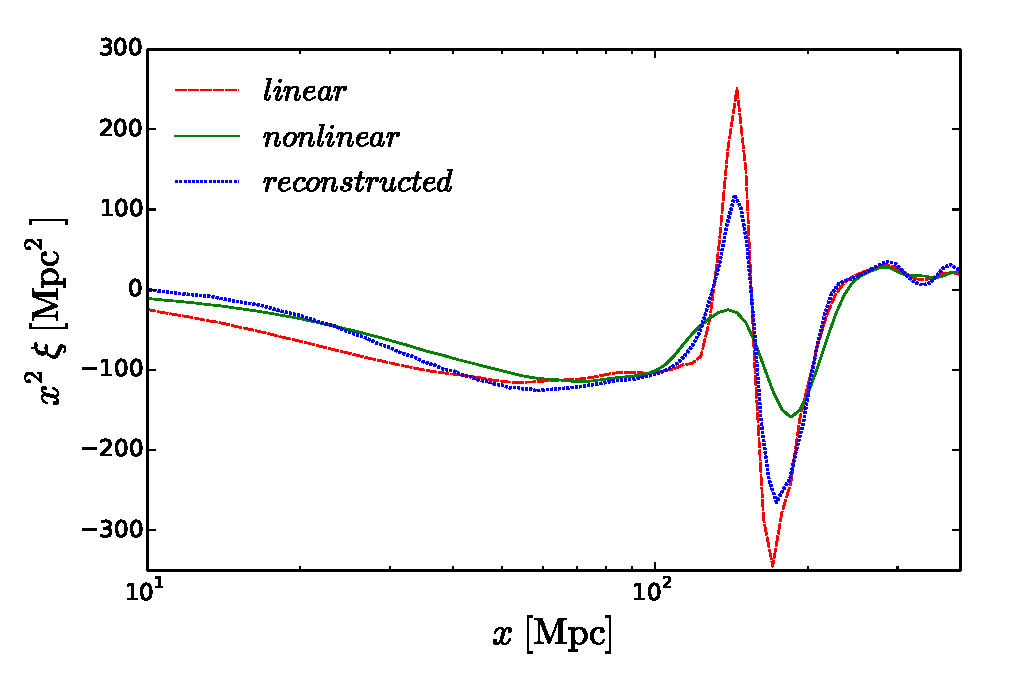
\includegraphics[width=0.48\textwidth]{f1.eps}
\end{center}
\vspace{-0.7cm}
\caption{The power spectra of the linear density field $\delta_L$, 
the nonlinear density field $\delta_\mr{NL}$ from the simulation, 
and the density field from Zeldovich approximation $\delta_\mr{ZA}$.}
\label{fig:ps}
\end{figure}

\section{Gaussianity and cross correlation}
The initial linear Gaussian density perturbations $\delta_L(\bm{x})$ 
evolve due to gravitational interaction. 
Given any initial linear density field, we have the evolved nonlinear density 
field $\delta(\bm{x})$ as a functional of $\delta_L(\bm{x})$,
\begin{eqnarray}
\delta(\bm{x})=F[\delta_L(\bm{x})],
\end{eqnarray}
where the gravtitational interaction process determines how the linear density
field $\delta_L$ is related to the nonlinear density field $\delta_\mr{NL}$.

We can easily decompose the nonlinear density field into two parts, 
\begin{eqnarray}
\delta(\bm{k})=b(\bm{k})\delta_L(\bm{k})+n(\bm{k}),
\end{eqnarray}
where $b(\bm{k})\delta_L(\bm{k})$ is correlated with the initial linear 
density field and $n(\bm{k})$ is generated in the nonlinear evolution.
Here, $b(\bm{k})$ is often called the ``propagator'' and $n(\bm{k})$ is usually
called the mode-coupling term \cite{2006crocce,2008crocce,2008matsubara}.
The mode-coupling term which arises from the nonlinear evolution contributes
as noises when we try to extract the information encoded in the linear density
field, like the positions of BAO peaks.

The propagator $b({k})$ and the noise term $n({k})$ can be evaluated 
easily from the correlations of the nonlinear field $\delta$ and the 
linear field $\delta_L$,
\bea
\langle\delta\delta_L\rangle=b\langle\delta_L\delta_L\rangle,\ \ \ 
\langle\delta\delta\rangle=b^2\langle\delta_L\delta_L\rangle+
\langle nn\rangle.
\eea
Note that $\delta_L$ has been rescaled using the linear growth function
to the same redshift as $\delta$. 
The propagator $b(k)$ and the noise power spectrum $P_n(k)$ is given by 
\bea
b({k})=\frac{P_{\delta\delta_L}(k)}{P_{\delta_L}(k)},\ \ \ 
P_n(k)=P_{\delta}(k)-b^2(k)P_{\delta_L}(k).
\eea
The cross-correltion coefficient of $\delta$ and $\delta_L$ is 
\bea
r(k)=\frac{P_{\delta\delta_L}(k)}
{\sqrt{P_{\delta}(k)P_{\delta_L}(k)}}
=\frac{1}{\sqrt{1+\eta(k)}},
\eea
where $\eta=P_n/(b^2P_{\delta_L})$.

In Fig. \ref{fig:ps2}, we plot the signal $b^2(k)P_L(k)$ and the noise 
power spectrum $P_n(k)$. The noise dominates over the signal when 
$k\gtrsim0.06/\mr{Mpc}$.

To solve the displacement field, we combine grids to get two fields with
five PM elements per grid and ten PM elements per grid, respectively.
In Fig. \ref{fig:ps7}, we show the power spectra with different number density.
We further get the reconstructed density field $\delta_r$ using the algorithm.
In Fig. \ref{fig:ps6}, we show the power spectra of $\delta_r$ and $\delta$.
In Fig. \ref{fig:ps8}, we show the power spectra of $\delta_r$ and $\delta_L$.

\begin{figure}[tbp]
\begin{center}
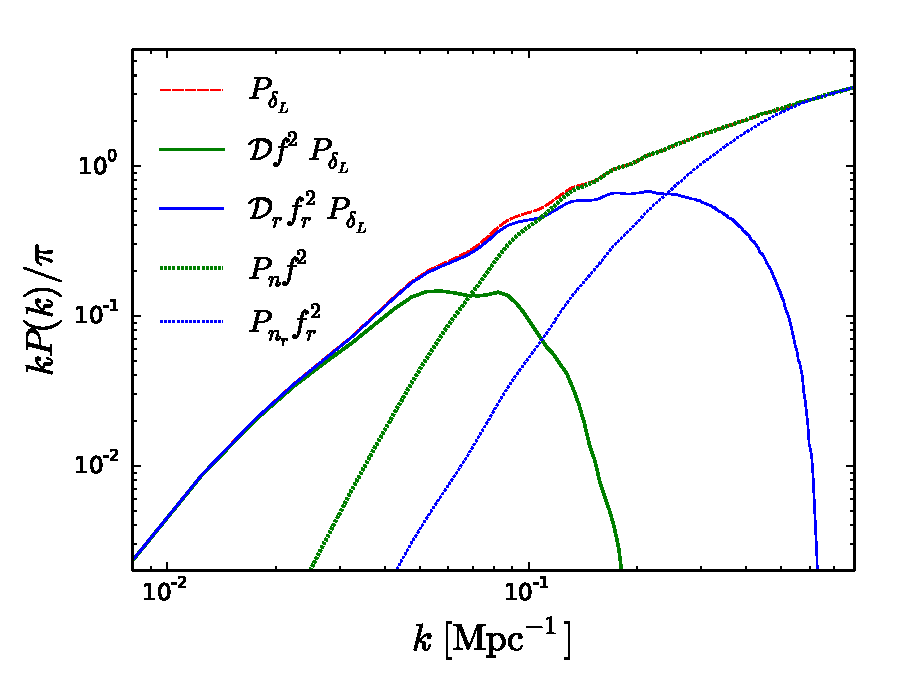
\includegraphics[width=0.48\textwidth]{f2.eps}
\end{center}
\vspace{-0.7cm}
\caption{The power spectra of $\delta_L$ and $\delta$. We also plot $b^2P_L$
and $P_n$. The noise dominates over the signal when $k\gtrsim0.06/\mr{Mpc}$.}
\label{fig:ps2}
\end{figure}

\begin{figure}[tbp]
\begin{center}
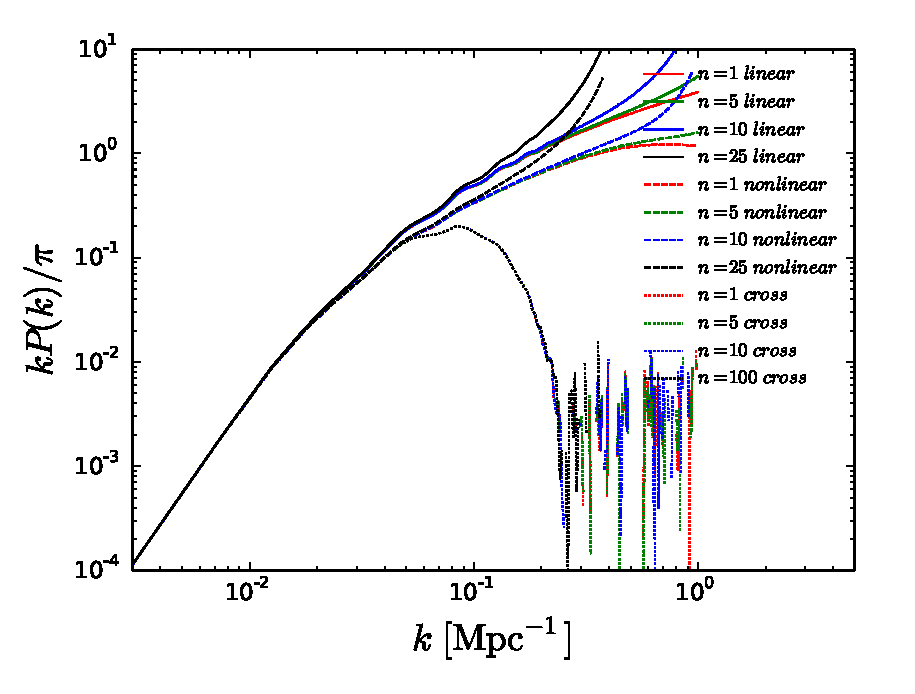
\includegraphics[width=0.48\textwidth]{f7.eps}
\end{center}
\vspace{-0.7cm}
\caption{The power spectra of $\delta_L$ and $\delta$ with $n=1/grid$ $n=5/grid$
and $n=10/grid$.}
\label{fig:ps7}
\end{figure}

\begin{figure}[tbp]
\begin{center}
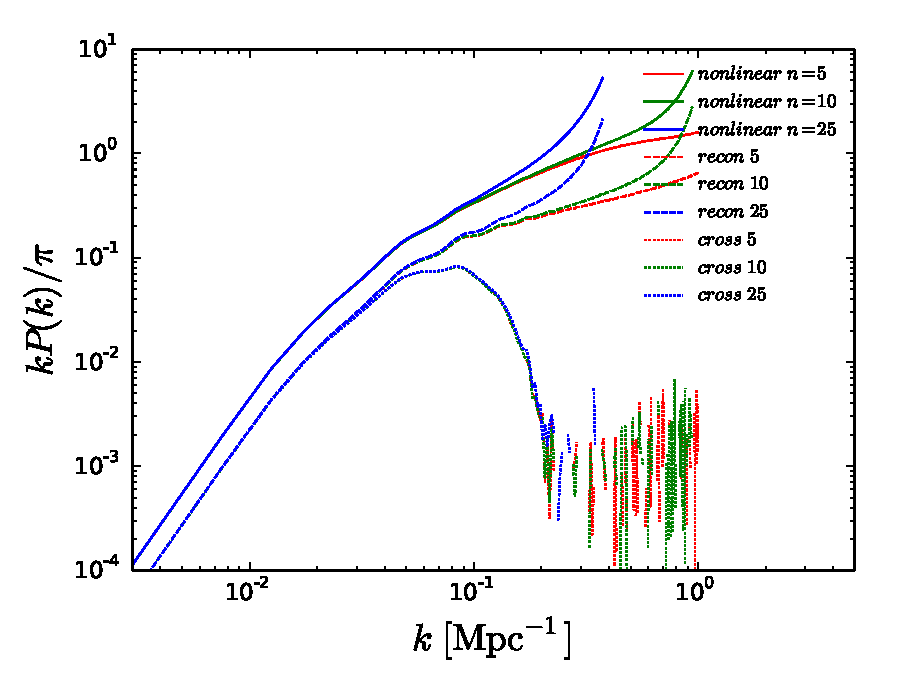
\includegraphics[width=0.48\textwidth]{f6.eps}
\end{center}
\vspace{-0.7cm}
\caption{The power spectra of $\delta_r$ and $\delta$ with $n=5/grid$
and $n=10/grid$.}
\label{fig:ps6}
\end{figure}

\begin{figure}[tbp]
\begin{center}
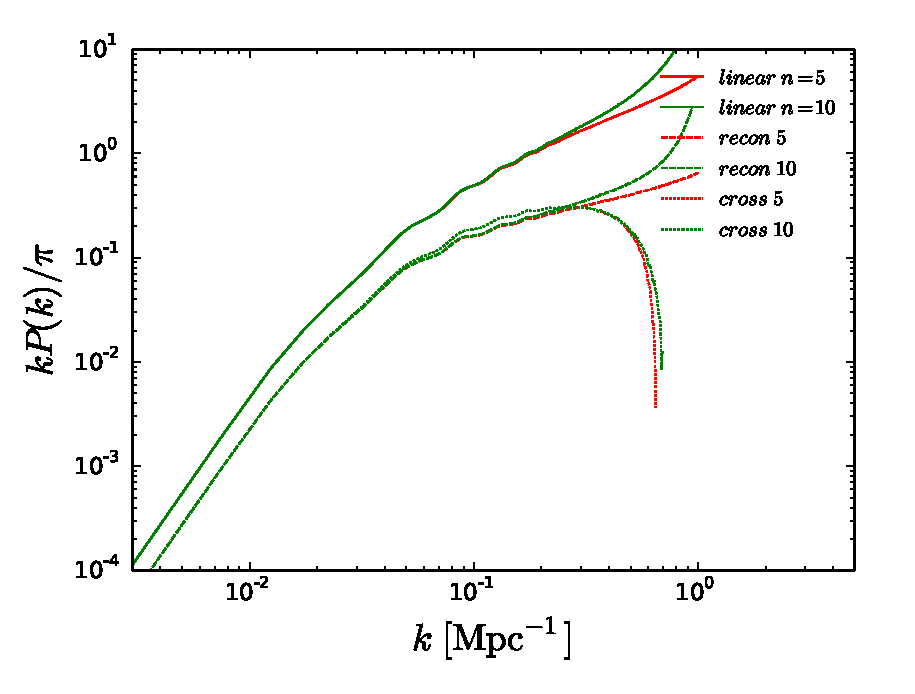
\includegraphics[width=0.48\textwidth]{f8.eps}
\end{center}
\vspace{-0.7cm}
\caption{The power spectra of $\delta_r$ and $\delta_L$ with $n=5/grid$
and $n=10/grid$.}
\label{fig:ps8}
\end{figure}




In Fig. \ref{fig:b}, we show the propagator $b(k)$ at $z=0$ and $z=10$.
In Fig. \ref{fig:xcc}, we show the cross-correlation coefficient at $z=0$ and 
$z=10$.

In Fig. , we show the distributions of the linear and nonlinear density 
fields.

\begin{figure}[tbp]
\begin{center}
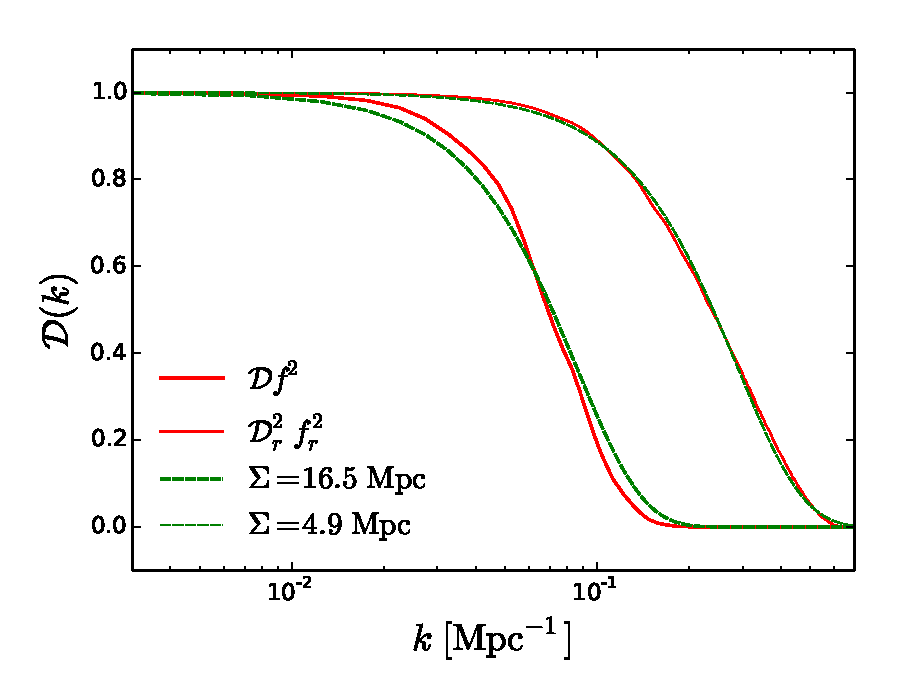
\includegraphics[width=0.48\textwidth]{f3.eps}
\end{center}
\vspace{-0.7cm}
\caption{The propagator $b(k)$ at $z=0$ and $z=10$.}
\label{fig:b}
\end{figure}


\begin{figure}[tbp]
\begin{center}
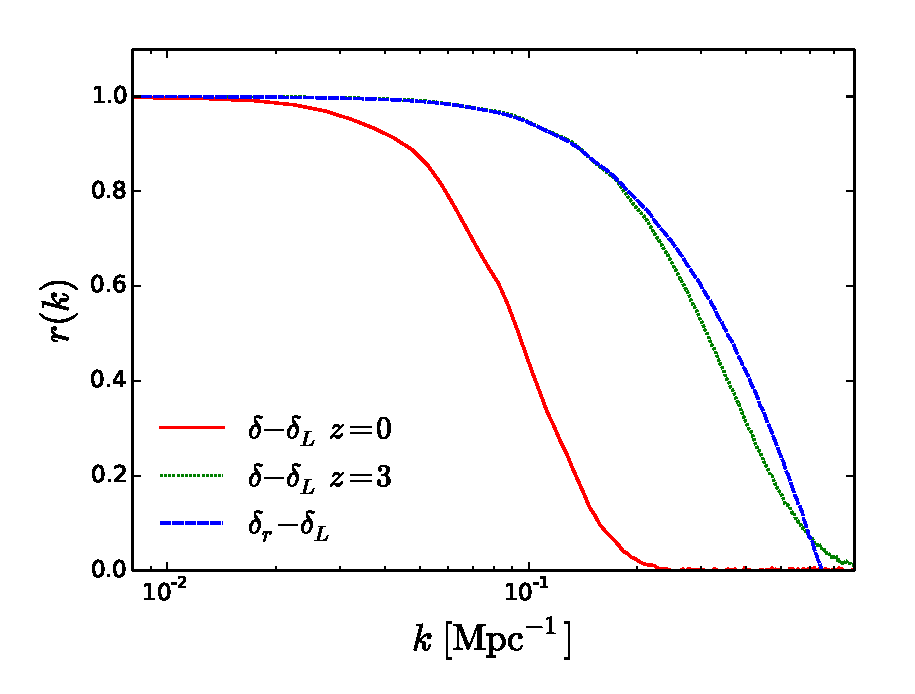
\includegraphics[width=0.48\textwidth]{f4.eps}
\end{center}
\vspace{-0.7cm}
\caption{The cross-correlation coefficient of $\delta$ and $\delta_L$ 
at $z=0$ and $z=10$.}
\label{fig:xcc}
\end{figure}

\begin{figure}[tbp]
\begin{center}
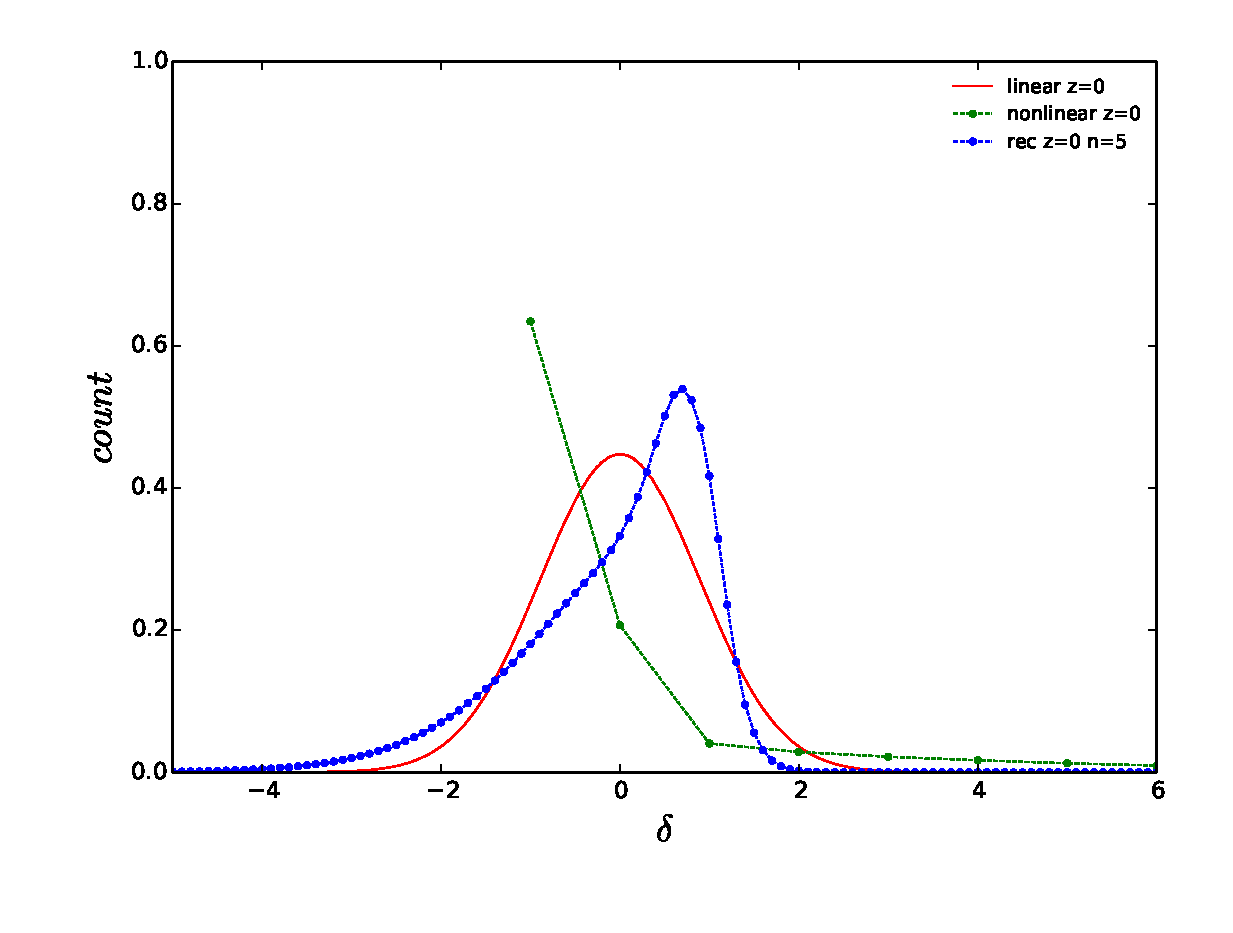
\includegraphics[width=0.48\textwidth]{f9.eps}
\end{center}
\vspace{-0.7cm}
\caption{The distributions of the density fluctuations. }
\label{fig:xcc}
\end{figure}


\subsection{Reconstruction}

\section{Covariance matrix and information content}

The covariance is calculated
using 100 simualtions and inormation content ...

Figure 3 covariance matrix for rec. Figure 4, covariance for BAO rec. Figure 5
information mode.

\section{Discussion}---This method can be generalized to the 3D case. We leave this
to future work.

\section{Acknowledgement}
We acknowledge the support of the Chinese MoST 863 program under Grant 
No. 2012AA121701, the CAS Science Strategic Priority Research Program 
XDB09000000, the NSFC under Grant No. 11373030, IAS at Tsinghua University, 
CHEP at Peking University, and NSERC.
The Dunlap Institute is funded through an endowment established by the David Dunlap family and the University of Toronto.
Research at the Perimeter Institute is supported by the Government of Canada
through Industry Canada and by the Province of Ontario through the Ministry of
Research $\&$ Innovation.

\bibliographystyle{apsrev}
\bibliography{1d}

\end{document}
